% TODO:
% 1. γιατί join(1000); Πού χρησιμεύει; το εγγραψα στο voip receive
\documentclass{article}
\usepackage{polyglossia}
\usepackage{amsmath}
\usepackage{fontspec}
\usepackage{lipsum}
\usepackage[margin=1in]{geometry}
\usepackage{graphicx}
\usepackage{caption}
\usepackage{subcaption}
\usepackage{hyperref}
\hypersetup{%
    colorlinks=true,
    linkcolor=blue,
    filecolor=magenta,      
    urlcolor=cyan,
    pdfinfo = {%
        Title = CN II VoIP over UDP
        Author = Χρήστος Μάριος Περδίκης, Αιμιλία Παλάσκα
        Producer = XeLaTeX
    }
}

% τι brewery παιχτηκε εδω
\NewDocumentCommand{\textsrcport}{}{\textit{text\_src\_port} $= 26555$}
\NewDocumentCommand{\textdestport}{}{\textit{text\_dest\_port} $= 26557$}
\NewDocumentCommand{\voicedestport}{}{\textit{voice\_dest\_port} $= 26567$}
\NewDocumentCommand{\voicesrcport}{}{\textit{voice\_src\_port} $= 26565$}

\title{CN\_II Chat and VoIP over UDP 2024}
%\author{\vspace{6pt}Ομάδα ΑΕ\\ 
    %Χρήστος Μάριος Περδίκης 10075 cperdikis@ece.auth.gr
   %\and Αιμιλία Παλάσκα 10453 aimiliapm@ece.auth.gr}
\author{\phantom{hehehe they will never see this coming!}Ομάδα ΑΕ\phantom{hehehe they will never see this coming!} \and 
    Χρήστος Μάριος Περδίκης 10075 cperdikis@ece.auth.gr
   \and Αιμιλία Παλάσκα 10453 aimiliapm@ece.auth.gr}
\date{}
% αν δεν δουλεύει αυτό το font άλλαξέ το, οποιοδήποτε .otf font με ελληνικούς χαρακτήρες will do
\setmainfont{FreeSerif}

\begin{document}
\maketitle
% περιγραφή κώδικα
% εικόνες ανταλλαγής κειμένου από Wireshark
% voice datagram stream από Wireshark

Το παρόν έγγραφο είναι η αναφορά της εργασίας του μαθήματος Δίκτυα Υπολογιστών 
ΙΙ. Κληθήκαμε να υλοποιήσουμε μια εφαρμογή VoIP και Chat σε Java η οποία θα
χρησιμοποιεί το πρωτόκολλο UDP. Συγκεκριμένα υλοποιήσαμε τον κώδικα αποστολής 
και λήψης πακέτων κειμένου και φωνής. Ακολουθεί η περιγραφή του κώδικα που γράψαμε.

\section{Ανταλλαγή μηνυμάτων κειμένου}
Λαμβάνουμε datagrams κειμένου στη θύρα \textdestport{} και στέλνουμε από τη θύρα 
\textdestport. Το μέγιστο μέγεθος του payload κάθε datagram είναι $1024$ bytes, αλλά όπως θα 
δούμε παρακάτω υποστηρίζουμε να σταλθούν μηνύματα μεγαλύτερου payload.

\subsection{Receive}
Ο μηχανισμός λήψης μηνυμάτων υλοποιείται στην συνάρτηση \textit{receiveText}.
Για να εγγυηθούμε ότι η λήψη πακέτων δεν θα περιορίσει την υπόλοιπη λειτουργικότητα της
εφαρμογής, δηλαδή την αποστολή μηνυμάτων και την δυνατότητα κλήσης, η συνάρτηση αυτή
ανατίθεται σε ένα Thread, το οποίο ξεκινάει από την main και εκτελεί μία αέναη λούπα. 
Μέσα σε αυτήν λαμβάνονται πακέτα ορισμένου μεγέθους ($1024$ bytes) και εμφανίζονται στην
διεπαφή, έχοντας σαν αρχή το ``Friend:'' για να γίνει αντιληπτό πότε πρόκειται για εισερχόμενο
μήνυμα.

Θεωρούμε ότι όλα τα πακέτα θα είναι το πολύ $1024$ bytes, διότι η διαδικασία
αποστολής μηνυμάτων διαχειρίζεται τον χωρισμό μεγάλων συμβολοσειρών σε πολλαπλά πακέτα.
Στην διάρκεια των δοκιμών μας δεν παρατηρήθηκε άφιξη των πακέτων με λάθος σειρά, όταν αυτά
προέρχονταν από χωρισμό μεγαλύτερου payload. 

\subsection{Send}
Αρχικά ελέγχουμε αν το \textit{inputTextField} είναι άδειο, στην οποία 
περίπτωση αγνοούμε το πάτημα του κουμπιού Send και δεν στέλνουμε τίποτα. 
Αν δεν είναι άδειο, τότε ξεκινάμε τη διαδικασία αποστολής ενός udp datagram.

Αφότου αποθηκεύσουμε το \textit{input\_text} στη μεταβλητή 
\textit{payload} σε μορφή bytes, υπολογίζουμε πόσες φορές χωράει το
$1024$ στο μήκος του \textit{payload}. Στη γενική περίπτωση, θα σταλθούν σε αριθμό
$\text{\textit{multiplier}} + 1$ datagrams, όπου όλα εκτός του τελευταίου
θα έχουν μέγεθος payload 1024 bytes και το τελευταίο θα έχει μέγεθος payload \textit{modulo}
bytes (\textit{multiplier} είναι το πηλίκο και \textit{modulo} το υπόλοιπο
της διαίρεσης $\text{\textit{payload.length}} / 1024$).

Για παράδειγμα, αν έχουμε ένα μήνυμα σε μέγεθος $2050$ bytes, το 
μήνυμα θα χωριστεί και θα σταλεί με δύο datagrams με payload μήκους $1024$ bytes
και ενός ακόμα datagram με payload μήκους $2050\ \%\ 1024 = 2$ bytes. Αν πάλι στείλουμε
ένα μήνυμα μεγέθους $256$ bytes, θα στείλουμε ένα payload μεγέθους $256$ bytes. Προφανώς
τα τελικά datagrams θα είναι λίγο μεγαλύτερα λόγω της προσθήκης του udp header.

\subsection{Παράδειγμα ανταλλαγής μηνυμάτων μέσω Wireshark}
Ακολουθούν ανταλλαγές μηνυμάτων κειμένου μεταξύ δύο υπολογιστών στο ίδιο δίκτυο 
οι οποίες καταγράφηκαν με το πρόγραμμα Wireshark. Οι διευθύνσεις IPv4 των δύο υπολογιστών
ήταν $192.168.100.22$ και $192.168.100.13$. Στην εικόνα~\ref{text-simple-n-small} βλέπουμε 
την αποστολή ενός μηνύματος με κείμενο ``hohoho''. Εφόσον έχουμε κείμενο μήκους $6$ bytes,
το datagram payload έχει και αυτό μέγεθος $6$ bytes.

\begin{figure}
    \centering
    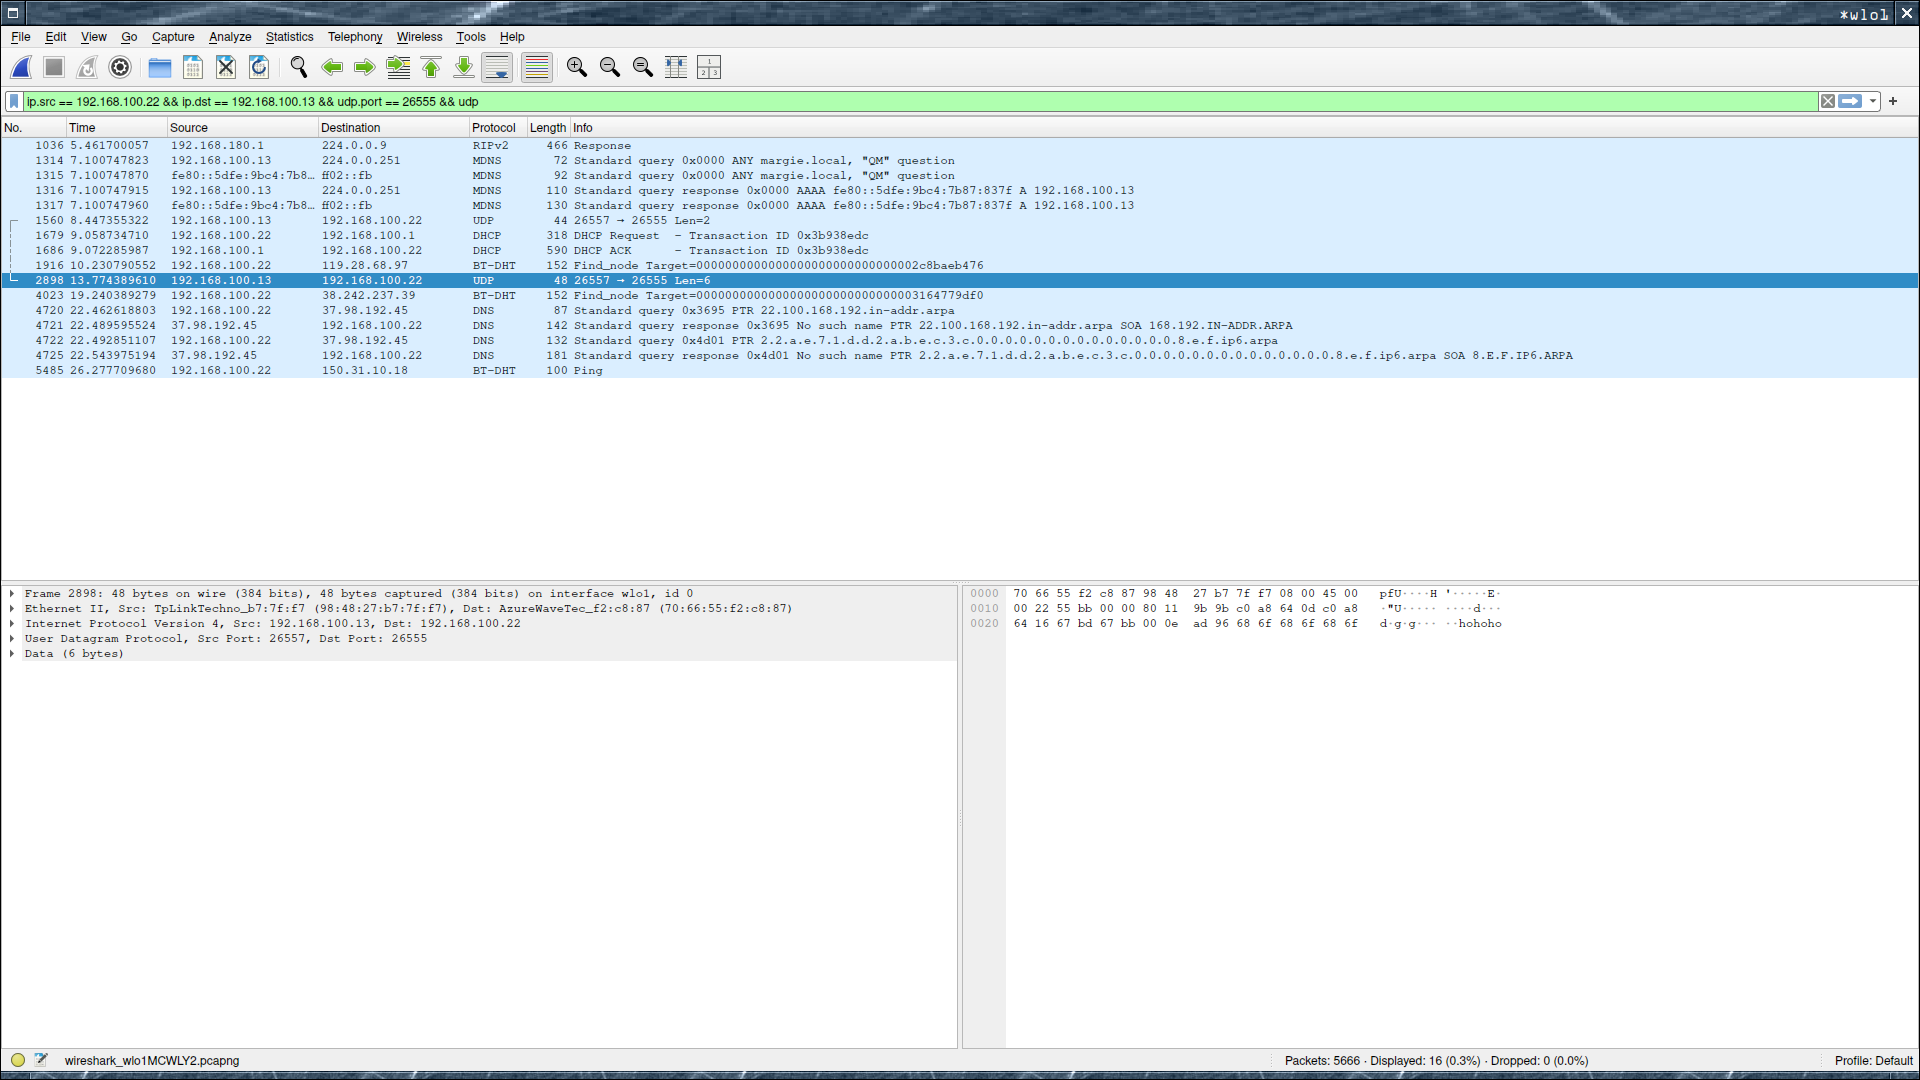
\includegraphics[scale=0.2]{text-simple-small.png}
    \caption{Καταγραφή μηνύματος μικρού μήκους στο Wireshark}\label{text-simple-n-small}
\end{figure}

Στις εικόνες~\ref{text-big},~\ref{text-big2} και~\ref{text-big-final} στείλαμε τον ίδιο 
τον πηγαίο κώδικα μέσω της εφαρμογής για να 
δοκιμάσουμε τη συμπεριφορά της σε πολύ μεγάλα κείμενα ($> 1024$ bytes). Βλέπουμε ότι το 
κείμενο χωρίζεται σε πολλά datagrams με μέγεθος payload $1024$ bytes μέχρι το τελευταίο
datagram στο οποίο στέλνεται ουσιαστικά ό,τι περίσσεψε.

\begin{figure}%
    \centering
    \subcaptionbox{Πρώτο datagram από πολλά που στάλθηκαν για να στείλουμε τον πηγαίο μας κώδικα!\label{text-big}}
        {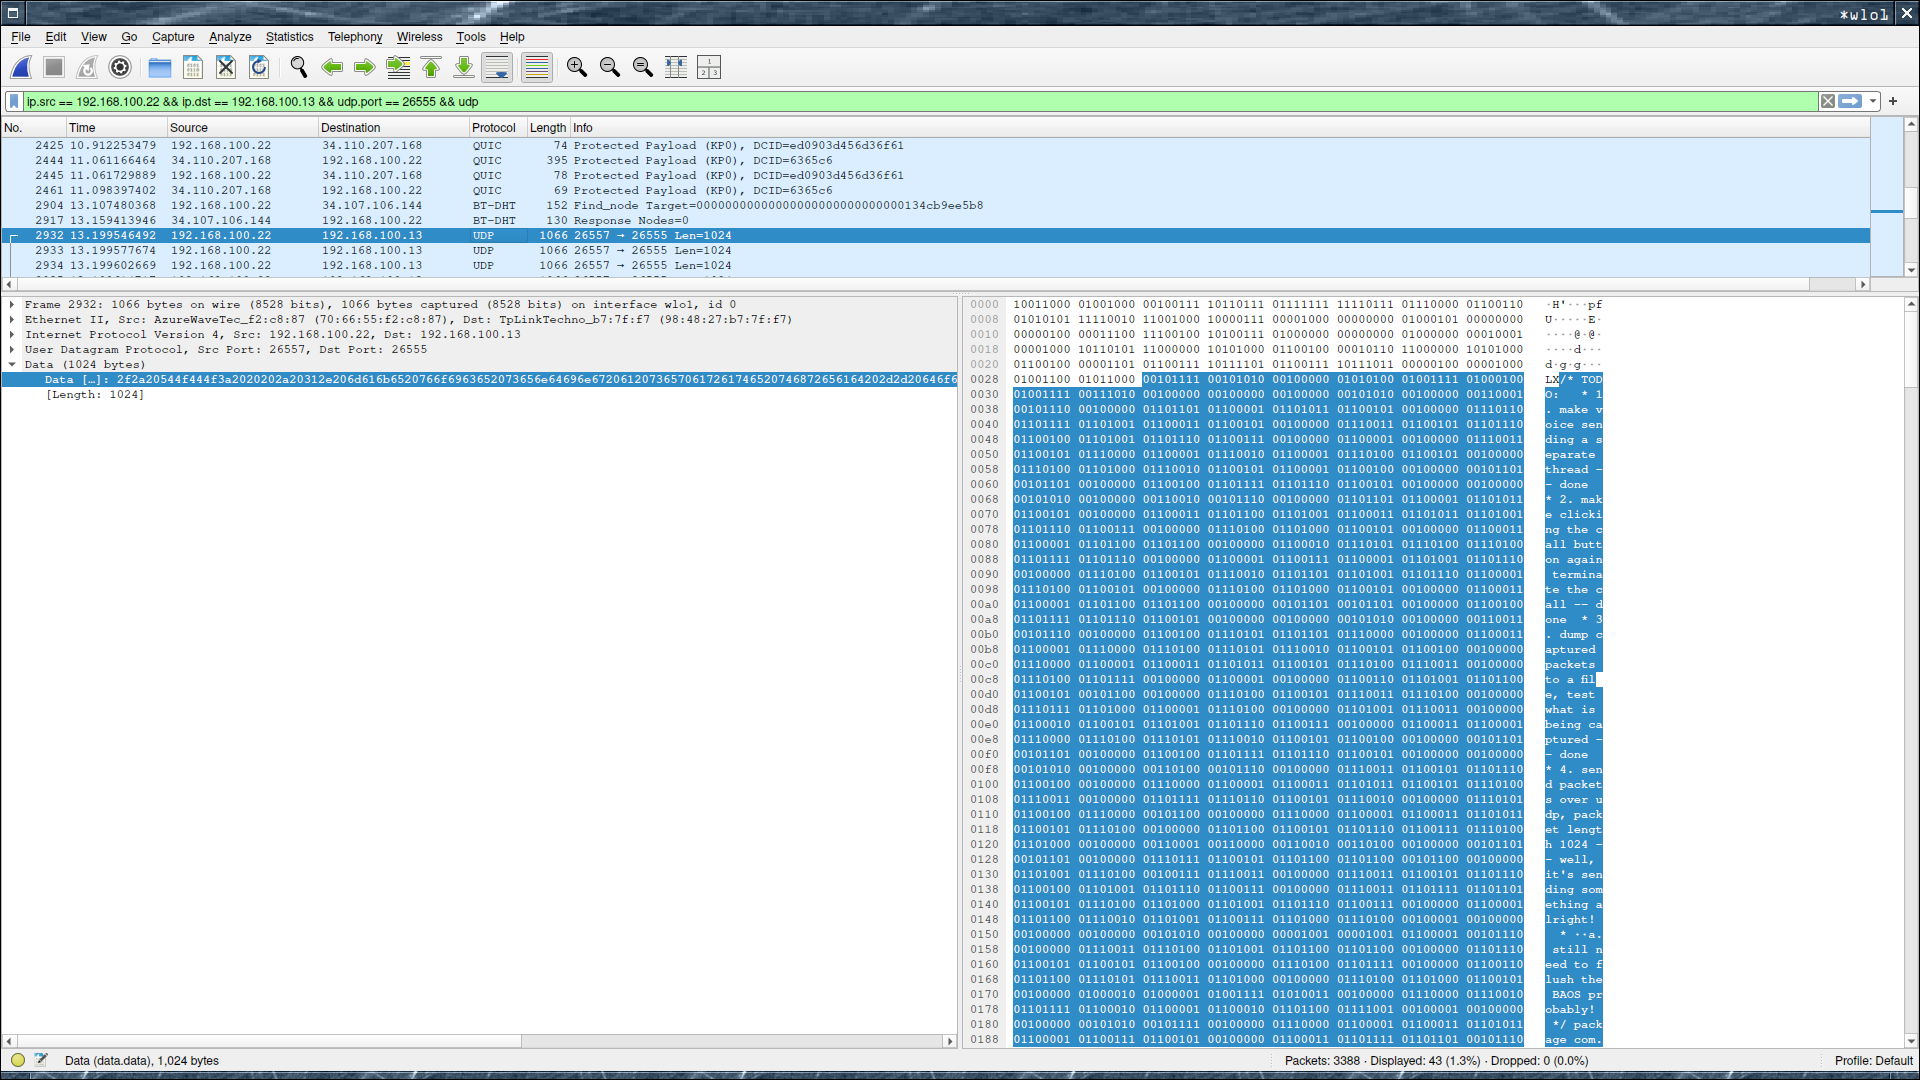
\includegraphics[scale=0.1]{textbigsend}}
    \subcaptionbox{Δεύτερο datagram. Όλα μέχρι και το προτελευταίο θα έχουν το ίδιο μήκος!\label{text-big2}}{%
        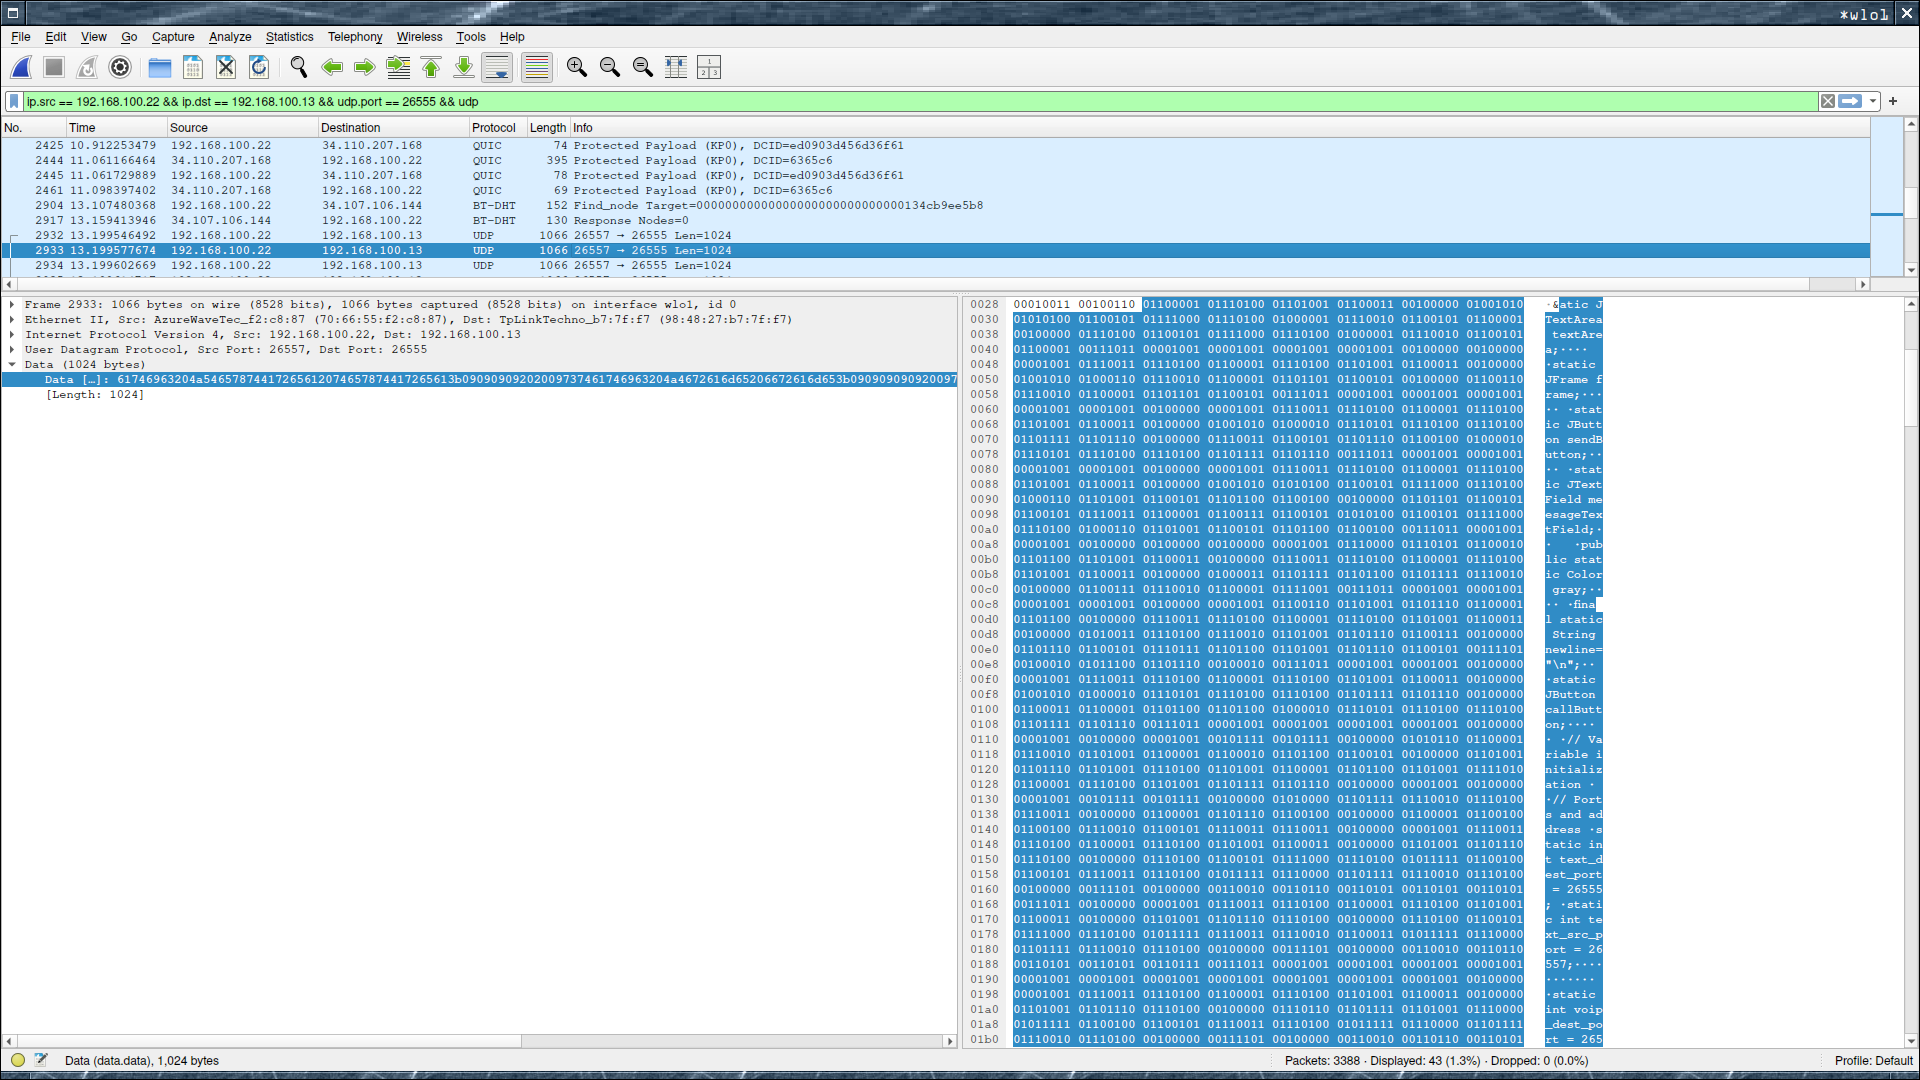
\includegraphics[scale=0.1]{text-big-send2.png}}
    \subcaptionbox{Τελευταίο datagram, μικρότερο σε μέγεθος από όλα τα προηγούμενα!\label{text-big-final}}{%
        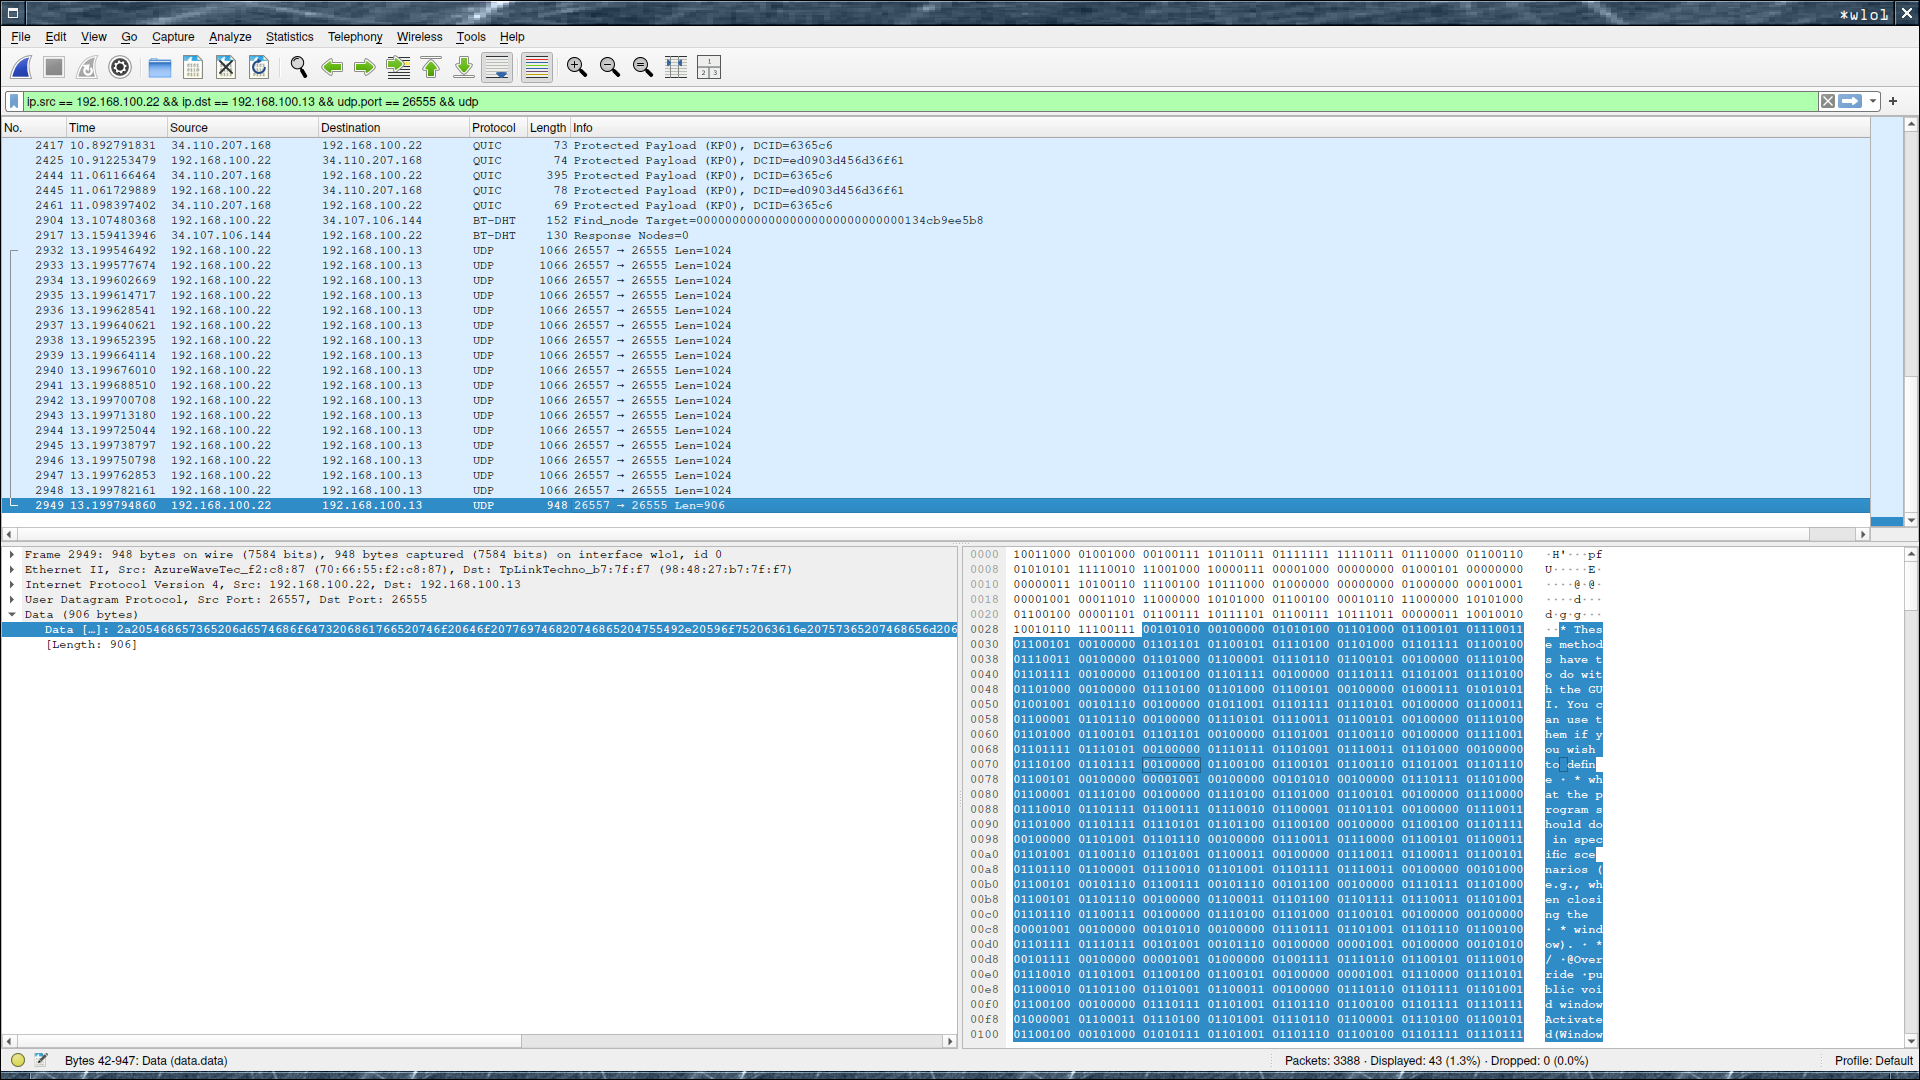
\includegraphics[scale=0.15]{text-big-send-final.png}}
        \caption{Καταγραφή αποστολής πολύ μεγάλου κειμένου με Wireshark}
\end{figure}


\subsection{Ερεύνηση του Maximum Transmission Unit}
Επιθυμούμε να βρούμε το Maximum Transmission Unit (MTU) του UDP. Γνωρίζουμε από τις διαλέξεις ότι θα είναι
περίπου $1500$ bytes. Θέτουμε ένα πολύ μεγάλο \textit{packet\_size} ($3000$ bytes) και στέλνουμε ένα μήνυμα 
μήκους $2962$ bytes. Σύμφωνα με τον κώδικά μας περιμένουμε να δούμε μόνο ένα UDP datagram.
Βλέπουμε από την καταγραφή σε Wireshark (\ref{mtu}) ότι το πακέτο μας τμηματίζεται αυτόματα σε πακέτα μέγιστου μήκους 
$1514$ bytes (payload και header). Στο τελευταίο πακέτο στέλνονται τα υπόλοιπα bytes και ανακατασκευάζεται το αρχικό μας κείμενο. 
Το κείμενό μας ανακατασκευάστηκε στον παραλήπτη καθώς από τη μεριά του φαίνεται σαν 
να λάβαμε μόνο ένα πακέτο. Άρα το MTU έχει payload $1480$ bytes.

Για αυτό το πείραμα χρησιμοποιήθηκαν υπολογιστές με διευθύνσεις $192.168.1.15$ και $192.168.1.30$. Έπειτα από
το πείραμα επαναφέραμε το \textit{packet\_size} σε $1024$ bytes. Για επαλήθευση, το κείμενο που στάλθηκε βρίσκεται
στο \href{https://github.com/PacoPacorius/diktya-II-ergasia}{GitHub repository} μας κάτω από τον φάκελο report
με όνομα \textit{mtu\_text}.

\begin{figure}%
    \centering
    \subcaptionbox{Πρώτο datagram έχει μήκος MTU, το ίδιο και το δεύτερο}
        {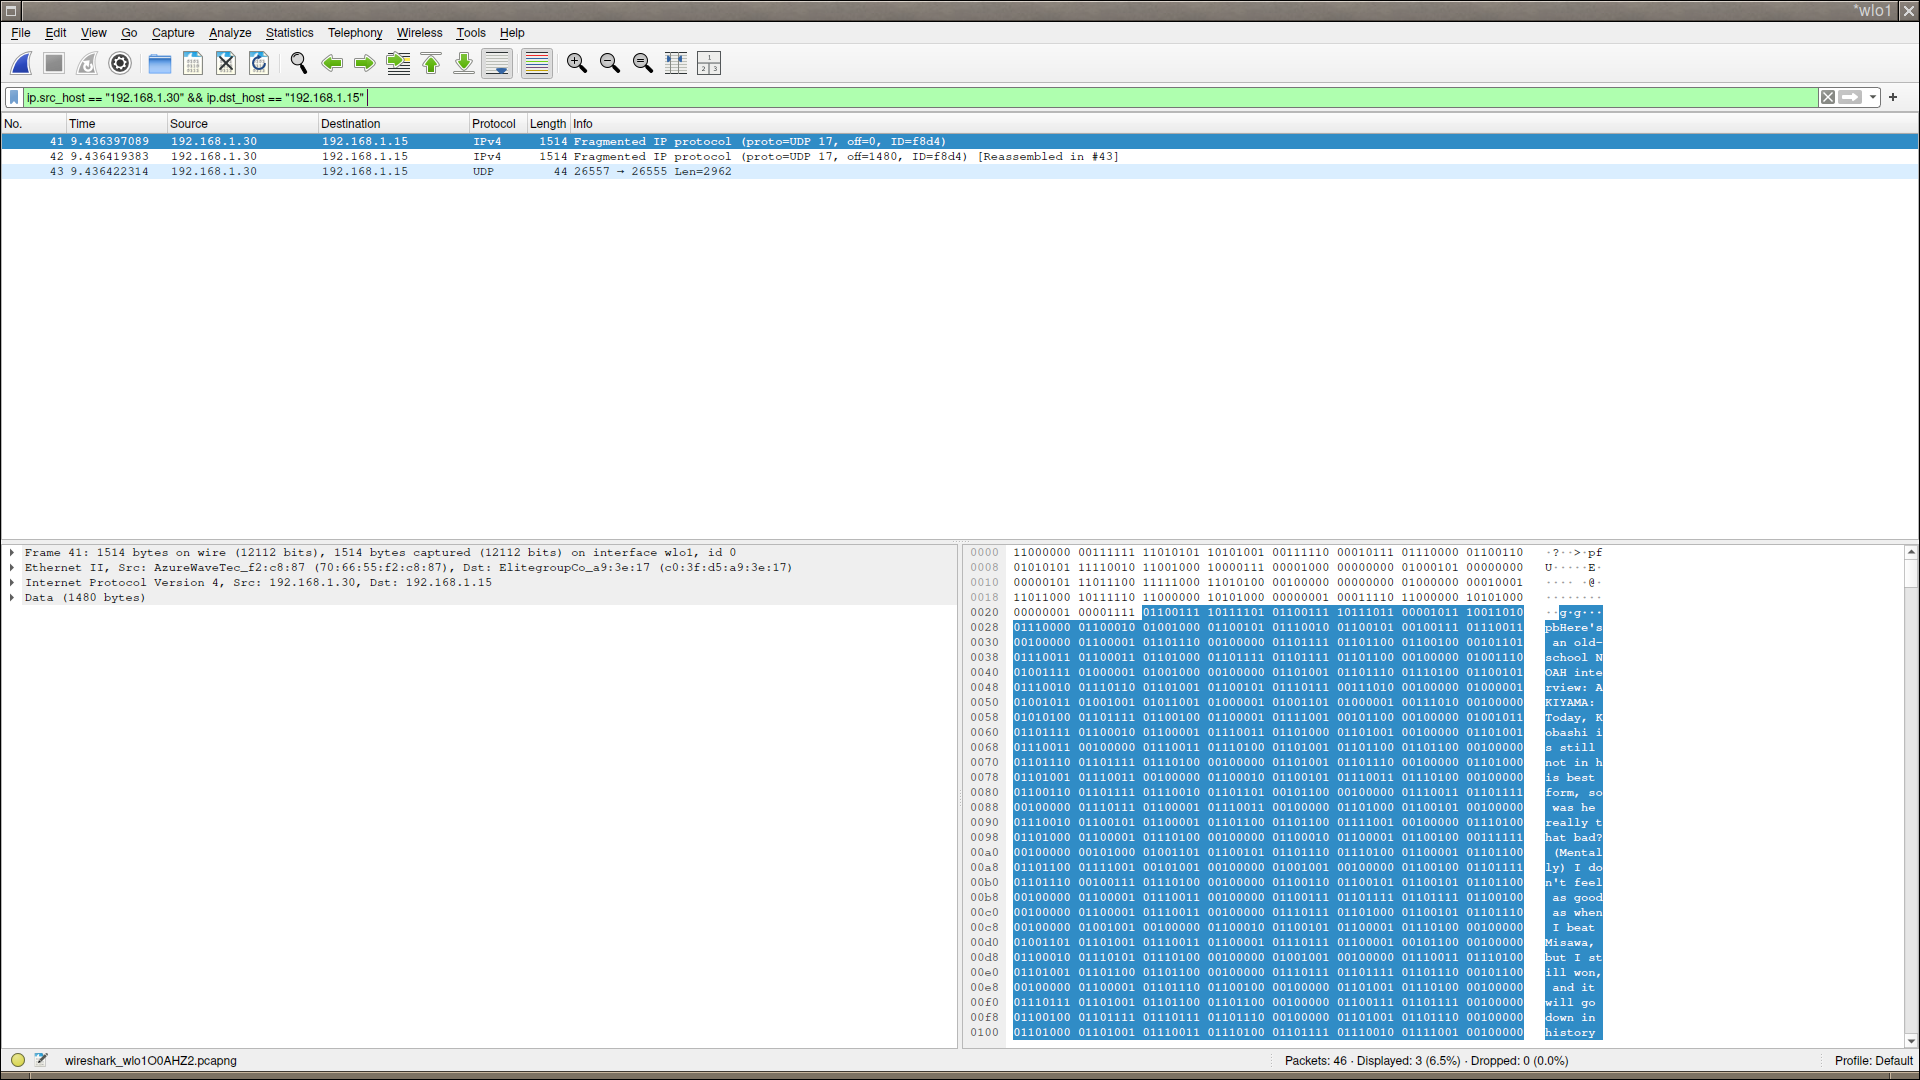
\includegraphics[scale=0.1]{mtu1.png}}
    \subcaptionbox{Τελευταίο datagram όπου στάλθηκε ό,τι περίσσεψε}{%
        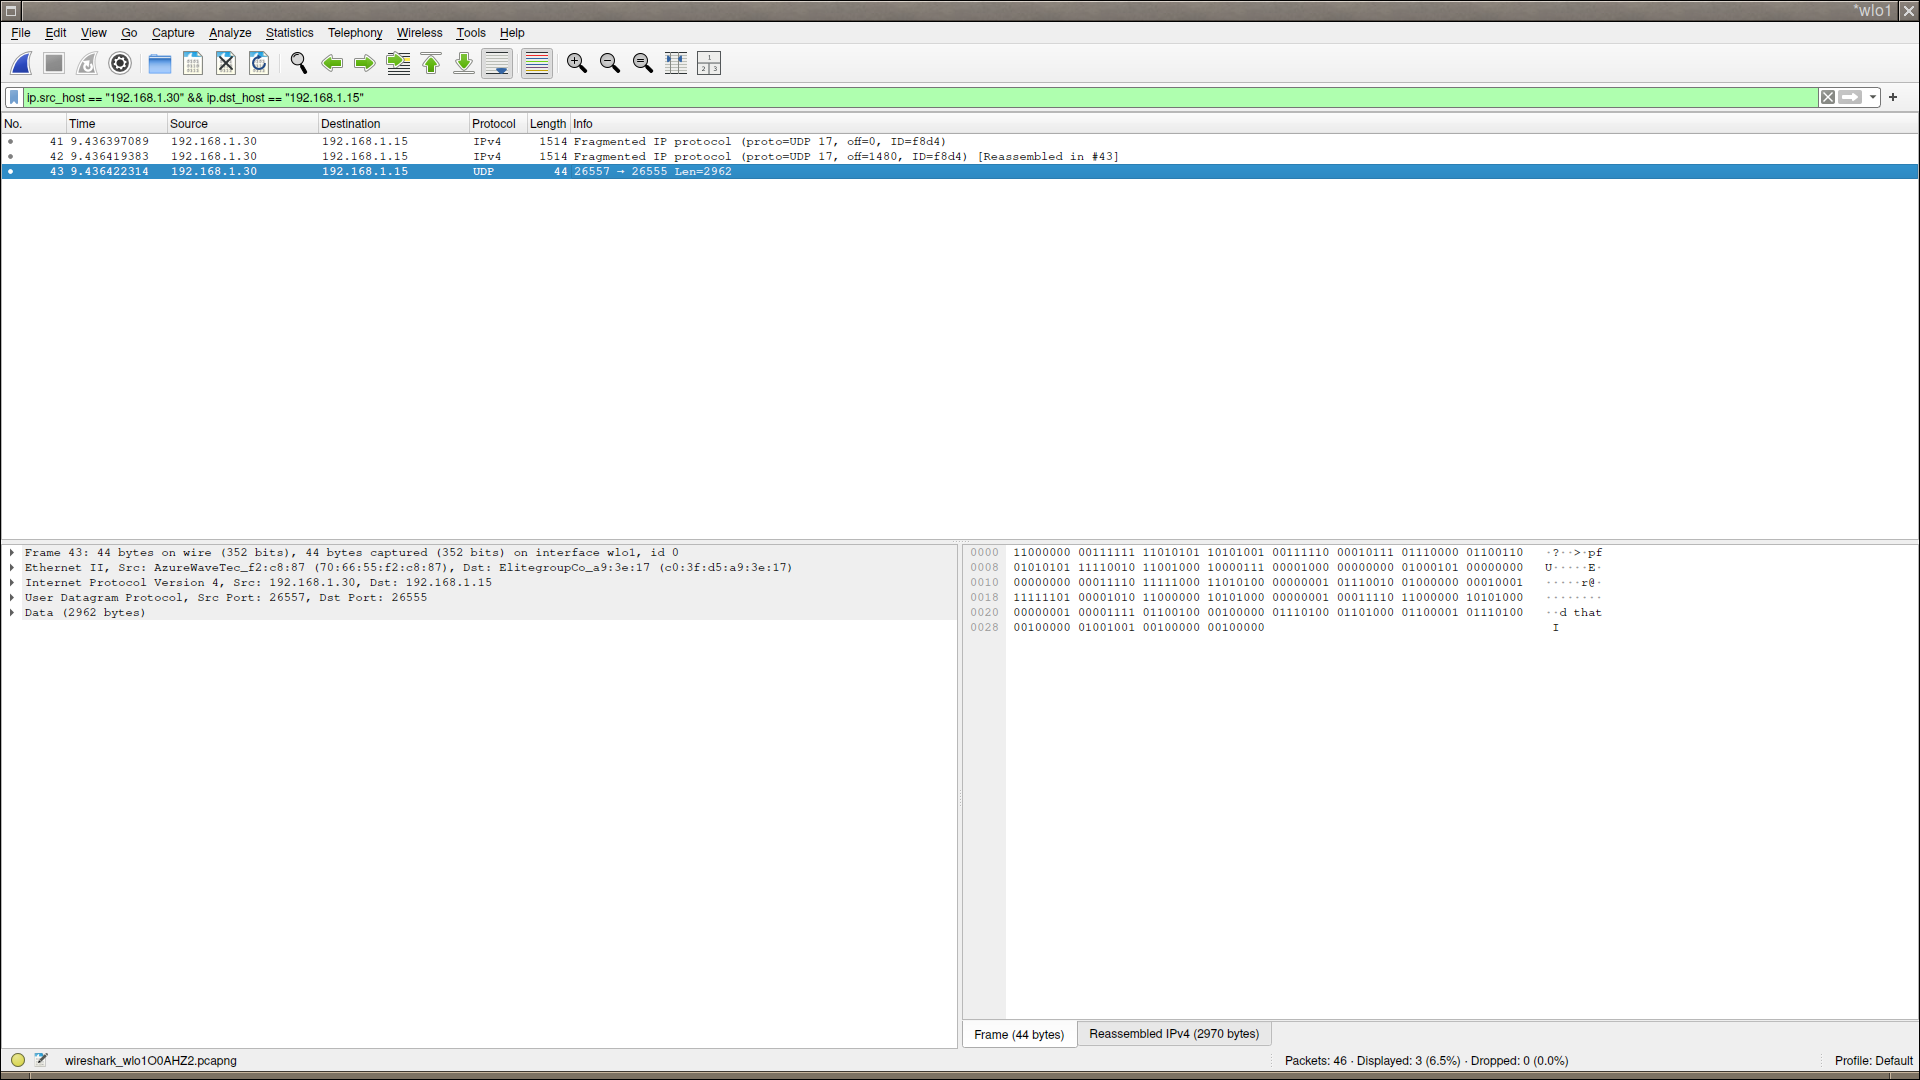
\includegraphics[scale=0.1]{mtu2.png}}
    \subcaptionbox{Ανακατασκευή του αρχικού κειμένου στον δέκτη}{%
        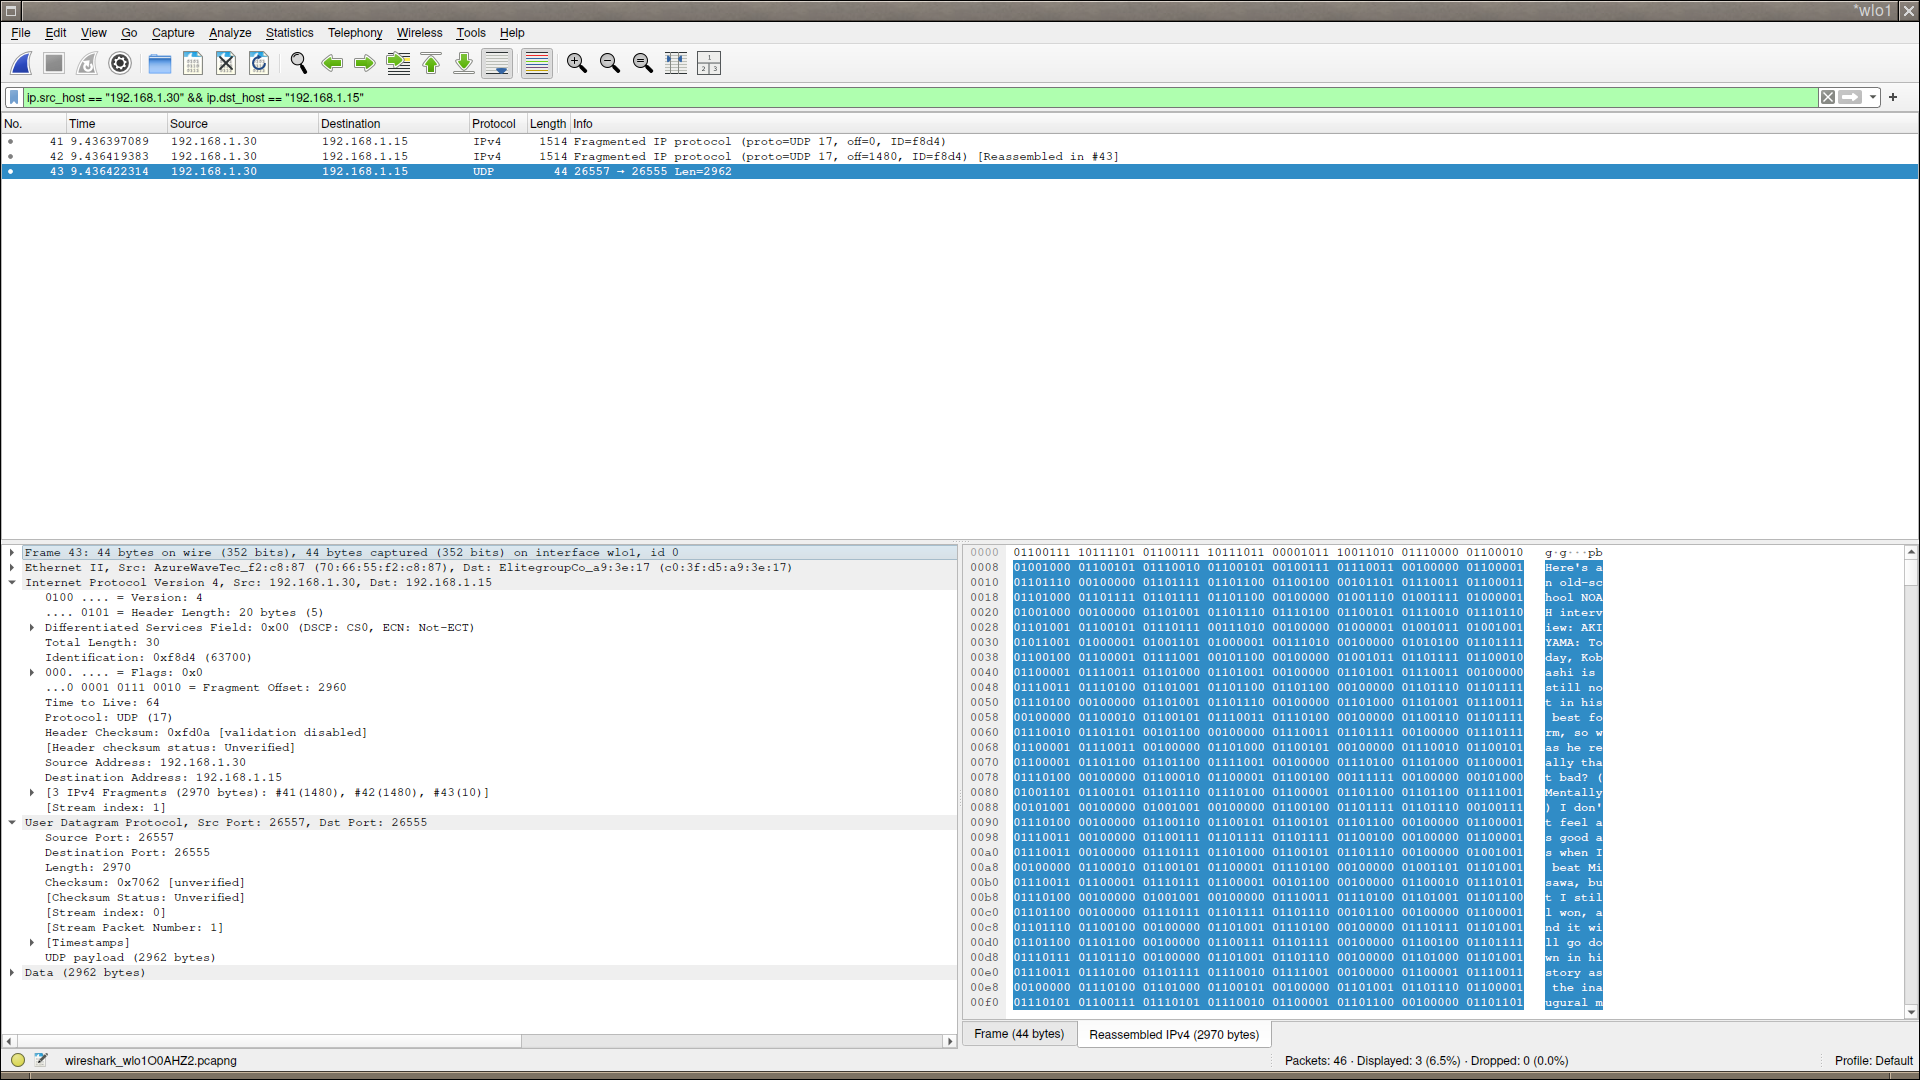
\includegraphics[scale=0.1]{mtu3.png}}
        \caption{Demonstration του UDP MTU σε δράση}\label{mtu}
\end{figure}

\section{VoIP}
Αντίστοιχα με λήψη και αποστολή κειμένου λαμβάνουμε datagrams φωνής στη θύρα \voicedestport{} και 
στέλνουμε από τη θύρα \voicesrcport. Το μέγεθος του κάθε πακέτου είναι σταθερό στα $1024$ bytes.
\subsection{Receive}
Κατά την εκκίνηση της κλήσης πρέπει να μπορούμε να δεχόμαστε και να αναπαράγουμε σύγχρονα, δηλαδή την στιγμή της
λήψης τους, πακέτα φωνής. Η διαδικάσία αυτή γίνεται στην συνάρτηση \textit{receiveVoIP} η οποία ανατίθεται σε ένα
thread και μπαίνει σε λειτουργία μετά το πάτημα του κουμπιού Call. 

Στην συνάρτηση, ανοίγουμε ένα \textit{DatagramSocket} το οποίο ``ακούει'' στην αντίστοιχη διεύθυνση και θύρα που
αναμένουμε να ληφθούν τα πακέτα. Εκτός από αυτό, αρχικοποιείται και ένα \textit{DataLine} το οποίο δέχεται πακέτα
ήχου με AudioFormat 8kHz μονοφωνικό PCM με 8-bits για κάθε sample. Παρόμοια με την λήψη μηνυμάτων, το νήμα εισέρχεται
σε μια ψευδο-αέναη λούπα, δηλαδή θεωρητικά τερματίζει όταν η μεταβλητή \textit{isCalling} γίνει False αλλά στην
πραγματικότητα η συνάρτηση receive του \textit{DatagramSocket} περιμένει επ'αόριστον την λήψη πακέτου, επομένως
αν σταματήσει η μετάδοση πακέτων η συνάρτηση μένει σε αυτήν την γραμμή και το νήμα παγώνει. Αυτό το φαινόμενο
οδηγήσε, κατά τις δοκιμές μας, την παρεμβολή ήχου μεταξύ των κλήσεων λόγω ανοιχτής και undrained γραμμής playback.

Για την επίλυση αυτού του προβλήματος παραλληλοποίησης κατά την διακοπή της κλήσης, δηλαδή όταν πατηθεί το κουμπί
Call αλλά διενεργείται ανταλλαγή πακέτων, διακόπτουμε (interrupt) απότομα τα νήματα.
Όμως θέλουμε να αποφύγουμε θόρυβο στο playback και προβλήματα δέσμευσης μνήμης, άρα περιμένουμε τα νήματα να σταματήσουν,
θέτοντας timeout  ενός δευτερολέπτου με την συνάρτηση \text{join(1000)}. Έπειτα, καλούμε 
την συνάρτηση \textit{receiveVoIPCleanup} η οποία διαχειρίζεται το playback line, αδειάζοντας το και κλείνοντας την 
μετάδοση ήχου, πετυχαίνοντας έτσι ένα αρκετά graceful exit. 

\subsection{Send}
% θεωρώ ότι αυτή η παράγραφος μπορεί να μπει πριν το receive
Aν πατήσουμε το κουμπί Call και δεν βρισκόμαστε σε κλήση, 
εκτός από το thread λήψης πακέτων φωνής, γίνεται εκκίνηση του thread καταγραφής και αποστολής φωνής.
Αν είμαστε ήδη σε κλήση, τότε τα δύο threads τερματίζουν ομαλά και η κλήση τελειώνει. Είναι δυνατή
η επανεκκίνηση της κλήσης αν πατηθεί το κουμπί Call ξανά.

Στο ξεχωριστό thread αναλαμβάνουμε την καταγραφή και την αποστολή ήχου. Με τις κατάλληλες ρυθμίσεις
στον υπολογιστή του χρήστη μπορεί να γίνει καταγραφή φωνής μέσω του μικροφώνου αλλά και καταγραφή των
ήχων του συστήματος όπως π.χ. μουσικής. Αφού αρχικοποιήσουμε το socket και την διεύθυνση του προορισμού,
θέτουμε το AudioFormat μας να είναι 8kHz μονοφωνικό PCM με 8-bits για κάθε sample. Αν είχαμε παραπάνω από 
ένα byte για κάθε sample, η διάταξή μας θα ήταν big endian. 

Ανοίγουμε ένα TargetDataLine με \mbox{\textit{buffer\_size} $= 1024$} και ξεκινάμε την καταγραφή ήχου
σε ένα while loop το οποίο τερματίζει μόνο όταν πατηθεί το κουμπί Call.
Κάθε φορά διαβάζουμε $1024/5 = 204$ bytes από τον εσωτερικό buffer του TargetDataLine, έτσι σιγουρευόμαστε
ότι δεν θα έχουμε ούτε buffer overflows ούτε underflows. Τα δεδομένα ήχου γίνονται append στο 
ByteArrayOutputStream \textit{out}, το οποίο μετατρέπουμε στο byte array \textit{audio\_data} όταν
θέλουμε να τα χρησιμοποιήσουμε.

Όταν το \textit{audio\_data} γεμίσει επαρκώς, τότε στέλνουμε ένα πακέτο. Αυτό γίνεται σειριακά με την
καταγραφή ήχου, στο ίδιο thread. Αν επιθυμούσαμε μικρότερο latency θα μπορούσαμε να είχαμε ξεχωριστά 
threads για την καταγραφή ήχου και την αποστολή πακέτων. Όταν το \textit{audio\_data}
συμπληρώσει $1024$ bytes, θα στείλουμε το πρώτο πακέτο το οποίο θα περιέχει τα πρώτα $1024$ bytes
του \textit{audio\_data}. Όταν συμπληρώσει $2*1024 = 2048$ bytes, θα στείλουμε $1024$ bytes με
offset $1*1024$ bytes από την αρχή του \textit{audio\_data}. Όμοια στα  $3*1024 = 3072$ bytes
θα στείλουμε $1024$ bytes με offset $2*1024$ bytes από την αρχή του \textit{audio\_data} κλπ.

Όταν το κουμπί Call πατηθεί όσο η κλήση βρίσκεται σε εξέλιξη φροντίζουμε να κλείσουμε τα TargetDataLine
και DatagramSocket μας για να μην έχουμε resource leaks. Μετά από αυτό, κυρίως για λόγους δοκιμών, 
αποθηκεύουμε σε ένα αρχείο ``test.wav'' τον ήχο που ηχογραφήθηκε και στάλθηκε (όχι τον ήχο που λάβαμε).

Υποθέτουμε ότι οι κλήσεις χρησιμοποιώντας 
αυτήν την εφαρμογή θα έχουν διάρκεια μερικών λεπτών ή μερικών ωρών, καθώς αφήνουμε το \textit{out} να μεγαλώνει 
ανεξέλεγκτα. Θεωρητικά αν περάσει επαρκής χρόνος τα \textit{out} και \textit{audio\_data} θα 
θα σταματήσουν να επεκτείνονται όταν το μέγεθός τους γίνει $Integer.MaxValue - 8$. Τότε το ByteArrayOutputStream θα 
εξακολουθεί να δέχεται νέα δεδομένα, επειδή όμως
στέλνουμε ένα νέο πακέτο κάθε φορά που μεγαλώνει το μέγεθος του \textit{audio\_data}, όταν αυτό φτάσει 
στο μέγιστο μέγεθος $Integer.MaxValue - 8$, η αποστολή των πακέτων ήχου θα σταματήσει. Με πρόχειρες 
μετρήσεις είδαμε ότι το BAOS \textit{out} μεγαλώνει κατά $10^4$ bytes περίπου κάθε $12$ δευτερόλεπτα. 
Υποθέτοντας ότι το BAOS \textit{out} αυξάνει σε μέγεθος γραμμικά, για να φτάσουμε στην μέγιστη τιμή ενός ακεραίου, 
την οποία θεωρήσαμε $10^9$ bytes για ευκολία στους υπολογισμούς, θα χρειαστούν περίπου $33$ ώρες. Θεωρούμε
ότι αυτό το χρονικό διάστημα είναι αρκετά μεγάλο έτσι ώστε να μην μας απασχολεί πότε θα φτάσουμε στο μέγιστο 
μέγεθος του BAOS. Όσο για τη χρήση μνήμης,
για κλήση μιας ώρας παρατηρήσαμε ότι το μέγεθος των \textit{out} και \textit{audio\_data} θα είναι περίπου $2 * 30 = 60$MB,
το οποίο δεν είναι πολύ μεγάλο νούμερο, άρα αναμένουμε η εφαρμογή μας να μην χρησιμοποιεί υπερβολικά πολύ
μνήμη τις πρώτες ώρες μιας κλήσης. Για αυτούς τους λόγους δεν επιχειρήσαμε να διορθώσουμε αυτό το πρόβλημα
παρόλου που γνωρίζαμε την ύπαρξή του. Μια εύκολη λύση θα ήταν να αδειάζαμε τα BAOS \textit{out} και το array
\textit{audio\_data} όταν έφταναν κάποιο προκαθορισμένο μέγεθος, όμως αυτό θα περιέπλεκε την αποθήκευση 
της ηχογράφησης σε αρχείο.


\subsection{Παράδειγμα VoIP μέσω Wireshark}
Στις εικόνες~\ref{voice-stream} και~\ref{voice-small-packets}, βλέπουμε την καταγραφή datagram φωνής από το Wireshark.
Δεν μπορούσαμε να έχουμε ορατά ολόκληρα τα payload και header του datagram την ίδια στιγμή με μέγεθος $payload = 1024$,
οπότε για τη δεύτερη φωτογραφία προσωρινά μικρύναμε το μήκος του payload σε $128$ bytes. Διευκρινίζουμε ότι το 
πρόγραμμά μας δεν δουλεύει με τον επιθυμητό τρόπο για payload των $128$ bytes. Δεν τροποποιήσαμε κανένα
άλλο κομμάτι του κώδικά μας, οπότε $1024 - 128 = 896$ bytes χάνονταν σε κάθε datagram που στέλναμε.
Ως αποτέλεσμα στη μεριά της λήψης ακουγόταν μόνο ένας ενοχλητικός θόρυβος. Η αλλαγή σε μικρότερου μήκους πακέτα 
έγινε μόνο για λόγους επίδειξης, ουσιαστικά για να χωρέσουμε ολόκληρο το datagram στην οθόνη.
Έχουμε επαναφέρει τον κώδικα ώστε να δουλεύει σωστά με $1024$ bytes στο payload του datagram.


\begin{figure}%
    \centering
    \subcaptionbox{Ροή datagrams ήχου\label{voice-stream}}
    {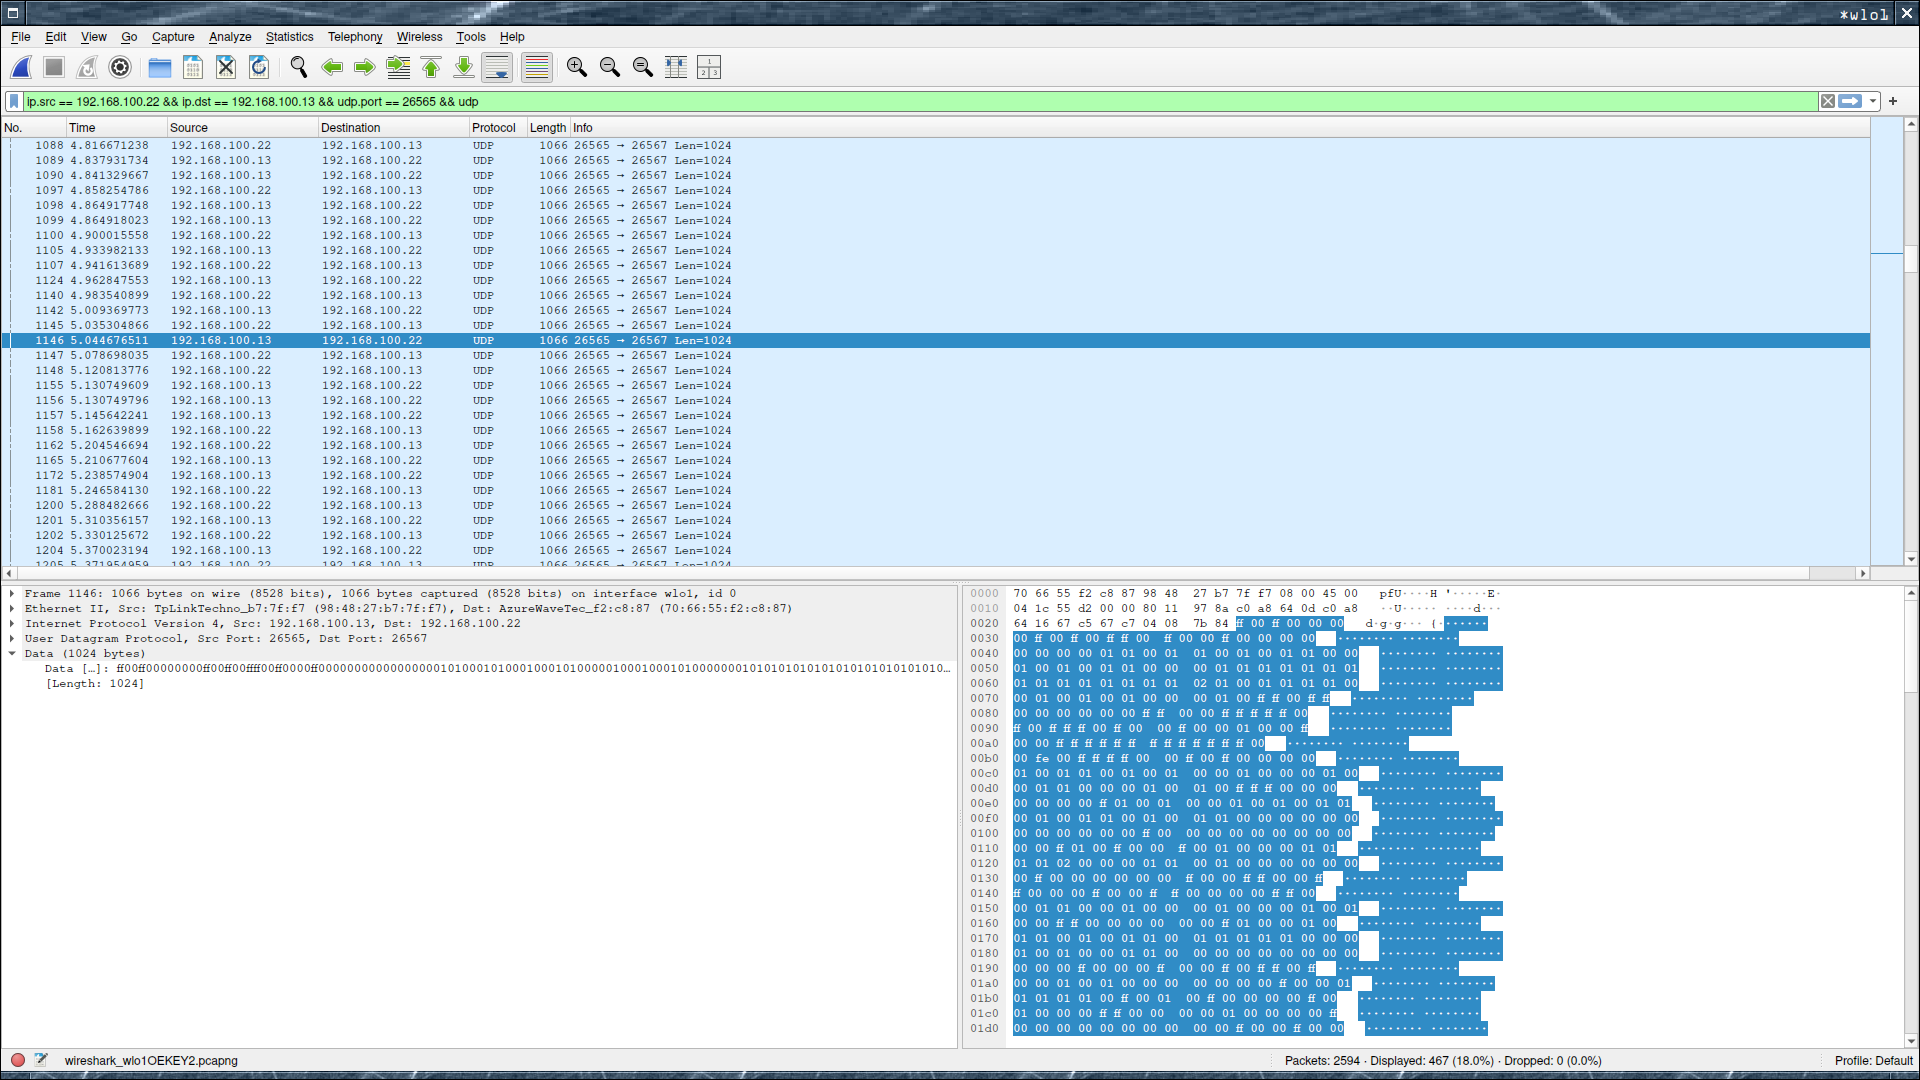
\includegraphics[scale=0.1]{voice-stream.png}}
    \subcaptionbox{Ροή datagrams ήχου όπου είναι ορατό όλο το header και όλο το payload\label{voice-small-packets}}
    {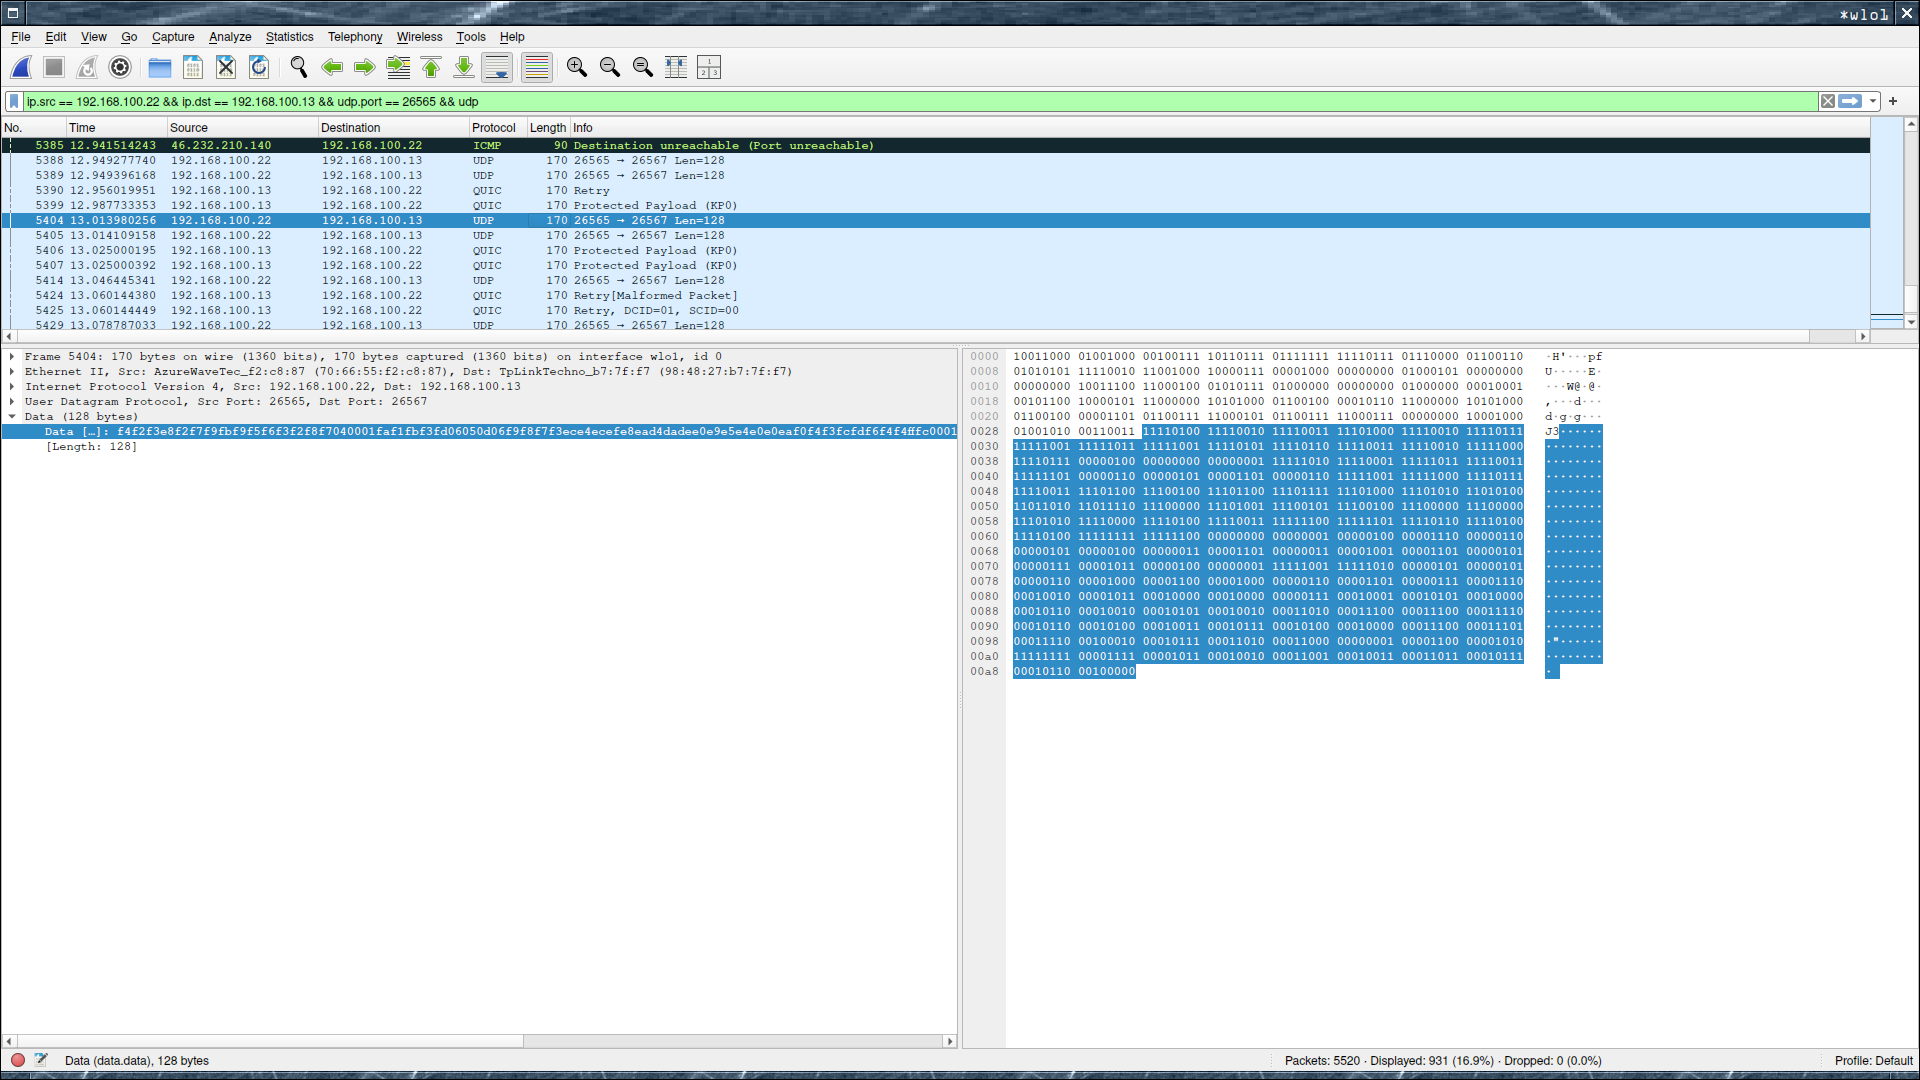
\includegraphics[scale=0.1]{voice-small-packets2.png}}
    \caption{Καταγραφή αποστολής πακέτων φωνής με Wireshark}
\end{figure}

\section{Κρυπτογράφηση}
Όπως αναφέραμε στο μάθημα, το πρωτόκολλο UDP δεν ακολουθεί κάποια διαδικασία κρυπτογράφησης ή πιστοποίησης της λήψης του πακέτου.
Επιλέξαμε για πειραματισμό να ενσωματώσουμε στην εφαρμογή μας το κομμάτι της κρυπτογράφησης στην αποστολή και λήψης μηνυμάτων κειμένου.
Επιλέξαμε για αυτό να χρησιμοποιήσουμε έτοιμες βιβλιοθήκες και συγκεκριμένα τις java.security και java.crypto. 
Ο αλγόριθμος κρυπτογράφησης που χρησιμοποιείται είναι ο \textit{AES} (Advanced Encryption Standard) σε λειτουργία \textit{CBC}
(Cipher Block Chaining) με padding \textit{PKCS5PADDING}.

Αυτό σημαίνει ότι:
\begin{itemize}
    \item Χρησιμοποιείται συμμετρική κρυπτογράφηση (ίδιο κλειδί για κρυπτογράφηση και αποκρυπτογράφηση) το οποίο δηλώνεται με την μεταβλητή
    \textit{AES\_KEY}. Αυτό είναι γνωστό από τους δύο end-users και δεν μπορεί να γίνει αποκρυπτογράφηση αν δεν είναι ίδιο και στις δύο εφαρμογές.
    \item Η λειτουργία CBC εξασφαλίζει ότι κάθε μπλοκ εξαρτάται από το προηγούμενο, προσφέροντας μεγαλύτερη ασφάλεια.
    \item Το padding PKCS5PADDING συμπληρώνει τα δεδομένα ώστε να έχουν μήκος πολλαπλάσιο του μπλοκ (16 bytes για AES). 
\end{itemize}

Η διαδικασία encryption και decryption γίνεται από τις υλοποιημένες συναρτήσεις \textit{encrypt} και \textit{decrypt}, ενώ οι βιβλιοθήκες παρέχουν
το μεγαλύτερο μέρος της λειτουργικότητας έτοιμο. Κατά τις δοκιμές μας έγινε προσπάθεια αποστολής μηνυμάτων χωρίς να είναι ίδια η παράμετρος
\textit{AES\_KEY}, με αποτέλεσμα αποτυχημένη αποκρυπτογράφηση δεδομένων. 

\newpage
\centering
\emph{*** ΤΕΛΟΣ ΑΝΑΦΟΡΑΣ ***}

\end{document}
